\documentclass[SE,lsstdraft,authoryear,toc]{lsstdoc}
% lsstdoc documentation: https://lsst-texmf.lsst.io/lsstdoc.html
\input{meta}

% Package imports go here.

% Local commands go here.

%If you want glossaries
%\input{aglossary.tex}
%\makeglossaries

\title{Operations Readiness Criteria}

% Optional subtitle
% \setDocSubtitle{A subtitle}

\author{%
Chuck Claver, 
Keith Bechtol, 
Robert Blum, 
Jim Bosch, 
Andrew Connolly, 
Leanne Guy,  
\v{Z}eljko Ivezi\'{c}, 
William O'Mullane; 
Add your name as you contribute
}

\setDocRef{SITCOMTN-005}
\setDocUpstreamLocation{\url{https://github.com/lsst-sitcom/sitcom-005}}

\date{\vcsDate}

% Optional: name of the document's curator
% \setDocCurator{The Curator of this Document}

\setDocAbstract{%
This document collects together the elements that constitute the criteria for completeness of the Rubin Observatory MREFC Construction Project,  DOE Rubin Observatory Commissioning, and the readiness for operations of the  Rubin Observatory to conduct the 10--year Legacy Survey of Space and Time (LSST).
\bigskip

This is a living document and will be modified and refined as required throughout the remainder of the Project.
\bigskip

In addition to this document and references therein, the completion of the Rubin Observatory Project will be evaluated based on the LSST Project Execution Plan (\citeds {LPM-17}) and the Commissioning Execution Plan (\citeds{LSE-390}).
}

% Change history defined here.
% Order: oldest first.
% Fields: VERSION, DATE, DESCRIPTION, OWNER NAME.
% See LPM-51 for version number policy.
\setDocChangeRecord{%
  \addtohist{1}{2020-08-06}{First draft}{Leanne Guy}
  \addtohist{1}{2020-08-10}{Revised version for internal review}{Chuck Claver}
  }


\begin{document}

% Create the title page.
\maketitle
% Frequently for a technote we do not want a title page  uncomment this to remove the title page and changelog.
% use \mkshorttitle to remove the extra pages

% ADD CONTENT HERE
% You can also use the \input command to include several content files.


\section {Introduction}

One of the primary high-level strategic inputs to developing the {\it System AI\&T and Commissioning Plan} (\citeds{LSE-79}) are the construction completeness requirements for the Construction Completeness Review (CCRs).  In (\citeds{LSE-79}), the Project has identified 10 general requirements for "construction completeness", including one requirement for "operations readiness", these are summarized as:

\begin{itemize}
        \item Verification of LSST System Requirements (\citeds {LSE-29}) and survey performance as described in SRD (\citeds {LPM-17})
        \item Verification of the Observatory System Specifications (\citeds {LSE-30})
        \item Verification of Data Processing, Products and User Services
        \item Demonstrating Science Data Quality Assessment (SDQA)
        \item Conduct a Science Validation Survey
        \item Demonstrate the system state is recorded and archived for each observation
        \item Verify Education and Public Outreach has met its requirements and construction scope
        \item Operational procedures and documented and accessible
        \item Provided a record of the as-built system, including modification since the as-build and non-compliance
        \item Demonstrate Rubin Operations Team readiness.
\end{itemize}

At the conclusion of the Rubin Observatory Construction Project's commissioning phase, a series of CCRs will be undertaken by an external panel jointly appointed by the DOE and NSF in consultation with the Project Team. The successful completion of the CCRs will signify the end of the NSF MREFC-funded construction project and DOE Commissioning. The CCRs are consistent with the NSF guidance given in the {\it Major facilities Guide} (\citeds{NSF-19-68}) Sections $2.4.2.1$ -- {\it Project Close--out Process}, $3.4.2.15$ -- {\it Commissioning}, $4.4$ -- {\it System Integration, Testing and Acceptance} and $4.5$ -- {\it Documentation Requirements}.

The series of CCRs will consist of four meetings, as shown in Figure XXX.
\begin{figure}[htbp]
\begin{center}
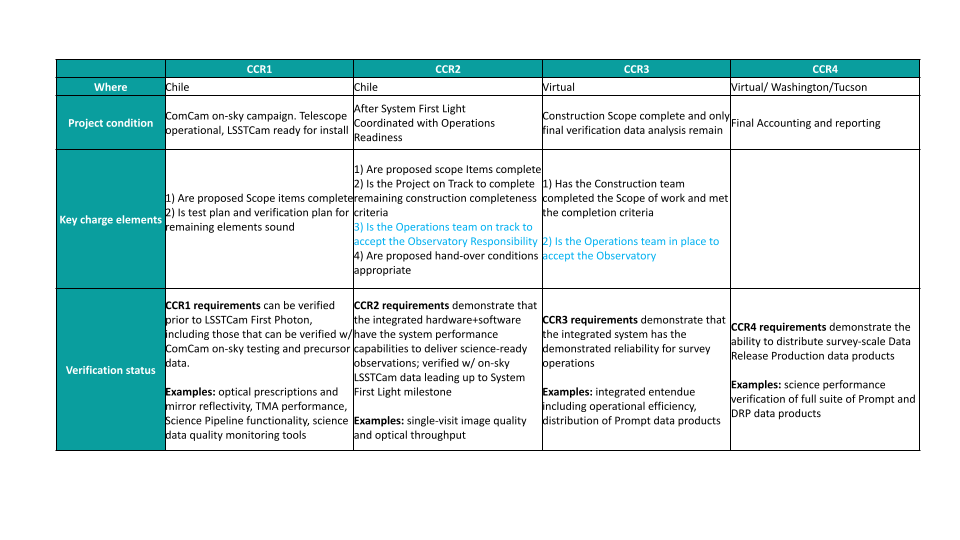
\includegraphics[width=1\textwidth]{./CCRs_overview.png}
\caption{Construction Completeness Review overview}
\label{CCRs_overview}
\end{center}
\end{figure}


The CCRs will cover two aspects: 
 1) The evaluation of the Rubin Construction Project completeness criteria and 
 2) the Rubin Observatory Operations team's readiness to receive the construction deliverables and begin planned operations for conducting the Legacy Survey of Space and Time -- the 10-year science survey for which the Rubin Observatory was designed and constructed to perform.

In this document, we collect together and detail the elements that constitute the criteria for construction completeness and operations readiness. 
Each topic has its own or will reference well-defined requirements -- in some cases, these include goals and stretch goals -- each will have the relevant supporting documentation for performance against the requirement. For those requirements that specify performance after some period of operations, the basis of the estimated projected performance will be provided. Unless otherwise specified, functional requirements will be verified by direct test, and performance requirements will be verified by direct test, analysis, or some combination thereof.  For each requirement, there will either be a clean pass or a waiver process that documents why it is acceptable to proceed to operations (or the reason we must postpone the transition to operations).

Some topics summarized in this document are already covered by existing verification plans.  Some functional requirements (and any accompanying goals and stretch goals) are still in review (at the time of this document version) -- in those cases, the requirements and associated verifications are being developed together to ensure clarity and crisp requirements for verifiability. Some topics, such as the Science Validation surveys, have requirements that are a combination of performance and functionality that do not easily flow directly from the high-level system requirements; in those cases, we identify the minimum requirements and performance that must be met to proceed to operations, along with a range of goals and stretch goals and the accompanying rationale.

For each of the general CRR requirements, we provide:

\begin{itemize}
	\item The statement of the requirements;
	\item An expansion of objective and intent;
	\item Specific criteria for completeness;
	\item Indication of any pre--Operation interactions; and
	\item The expected delivered artifacts.
\end{itemize}
	
\section{Observatory System Specifications (LSE-30) Verifcation}  \label{sec:oss}

\subsection{Operations Readiness Requirement}
The project team shall demonstrate that the integrated LSST systems (Camera, Telescope \& Site and Data Management subsystems) as well as the Education and Public Outreach (EPO) system have met the technical specifications enumerated in the LSST Observatory System Specifications (\citeds {LSE-30}).

\subsection{Objectives}

The main objective with this Operations Readiness Requirement is to verify the system specifications in the OSS (LSE-30) are proven and well documented..  The OSS is essentially the highest level document describing the basic LSST system technical architecture.  It contains sections derived from the OSS on the following broad topics:

\begin{itemize}
\item System Composition and Constraints

\item Common System Functions and Performance, including:

	\begin{itemize}
		\item System Control
		\item System Monitoring and Diagnostics
		\item System Maintenance
		\item System Availability
		\item System Time References
	\end{itemize}

\item Detailed Specifications:

	\begin{itemize}
		\item Science and Bulk Data
		\item Optical System
		\item System Throughput
		\item Camera System
		\item Photometric Calibration
		\item System Timing and Dynamics
	\end{itemize}
	
\item Education and Public Outreach

\end{itemize}

\subsection{Criteria for Completeness}
Compliance with this objective will follow the process as defined in the Verification and ValidationProcess document (LSE-160) and associated documentation.   All technical specifications in the OSS (LSE-30) and LSR (LSE-29) are expected be met at the end of construction.

\subsection{Pre--Operations Interaction}
None.  Unless there are non-compliance issues against the ORR requirements and specifications.

\subsection{Artifacts for Completion}

\begin{itemize}
 
	\item Verification matrix containing entries for all OSS requirements and specifications.  Methods, inspections, demonstration, analysis or test, shall be identified for every OSS requirement.  Final compliance status will be included.

	\item Analysis reports where the verification method has been identified as "test" or "analysis".
	\item Non-compliance reports.

\end{itemize}
\section{LSST System Requirements \& SRD Verification/Validation}  \label{sec:srd}

\subsection{Operations Readiness Requirement:}

The Project team shall characterize and document the performance of the integrated LSST system with respect to the survey performance requirements and specifications enumerated in the LSST System Requirements, Observatory System Specifications and Science Requirements Document (LSE-29, LSE-030, \& LPM-17 Section 3, respectively);

\subsection{Objectives:}

The primary objective for this Construction Completeness Requirement is to verify and validate that the data produced from the Science Validation surveys (and any additional observing campaigns) meets the science verification requirements as described in the LSST Verification and Validation (LVV) elements and test cases. System-level requirements include

\begin{itemize}
\item Verification of the generation of all required data products and services;
\item Verification that the relevant metadata are being collected and archived;
\item Verification of astrometric performance (relative and absolute);
\item Verification of photometric performance (relative and absolute);
\item Verification of data throughput and processing requirements for prompt data products;
\item Completeness and purity of sources detected in AP and DRP;
\item Object deblending;
\item Image template generation;
\item Completeness and purity of moving object orbit calculations;
\item The impact of stray light and optical ghosts;
\item Image quality (defined for each subsystem: telescope, camera, data management);
\item Crosstalk, filter response, and calibration.
\end{itemize}

In addition to the normative data quality metrics above, there are several science validation and characterization objectives that represent important benchmarks of scientific capability. The optimization of associated algorithms is in many cases an active research topic, and performance is expected to improve throughout Operations. Science validation studies include:

\begin{itemize}
\item Object classification (e.g., for star-galaxy separation);
\item Galaxy photometry (e.g., for photometric redshifts);
\item Difference image analysis photometry (e.g., for statistical variability metrics);
\item Low surface brightness features;
\item Shear calibration and weak-lensing null tests for galaxies; and
\item Treatment crowded fields.
\end{itemize}

Verification and validation of high-level science performance will make use of Quality Assessment (QA) and Quality Control (QC) tools developed during DM construction.

\begin{itemize}
\item Quality Assessment: versatile pipelines to calculate performance metrics and other diagnostics
\item Quality Control: ensure that metrics are routinely calculated and track their distributions as the pipelines evolve and encounter new data
\end{itemize}

In particular, Key Performance Metrics produced by DM and the Commissioning team, together with additional test cases, will be compared against the tabular requirements in the LSST SRD. 

\textbf{Discussion}

For the purpose of evaluating readiness, we define the following steps associated with verification, validation, and characterization of the LSST data and processing.

\emph{Verification}: Demonstrate that the system as built is consistent with the design. Ensure that the requirements for the system are met using LSST and precursor data. Express the requirements in terms of metrics that can be evaluated using LSST and precursor data. Document the system performance for each of the verification metrics and requirements.

\emph{Validation}: Demonstrate that the system is capable of meeting the scientific objectives of the survey. Ensure that the data products, data access, and science requirements can meet the objectives for LSST?s four major science themes. Document the system performance for each of the validation metrics and requirements and verify that there exist mechanisms to monitor the system performance during operations. Validate that the derived data products and access tools meet the science requirements of the community.

\emph{Characterization}: Determine how the performance of the system degrades as a function of environment and technical performance of the components of the system. Measure how the metrics used in verification change as a function of operational conditions (including weather, site, operations, telescope, instrument, and software).

The scope of science verification and validation activities includes:

\begin{itemize}
\item Determining whether the specifications defined in the OSS, LSR, and SRD are being met;
\item Characterizing other system performance metrics in the context of the four primary science drivers;
\item Studying environmental dependencies and technical optimization that inform early operations;
\item Documenting system performance and verifying mechanisms to monitor system performance during operations; and
\item Validating data delivery, derived data products, and data access tools that will be used by the science community.
\end{itemize}

The goal is to quantify the range of demonstrated performance by using a combination of on-sky data, informed simulations of the LSST system, and external datasets. Observations taken during this period will enable higher-level data quality assessments that are not explicitly identified as requirements in the LSR or SRD, but nonetheless represent important benchmarks of scientific performance (e.g., source detection completeness, accuracy of star-galaxy separation, precision of photometric redshifts, and weak-lensing null tests). 

All test cases as described under the LSST Verification and Validation project will be implemented as either part of the DM Key Performance Metric validation system, as separate test procedures (e.g., Jupyter notebooks), or via visual inspection (e.g., to demonstrate that a service or data produce has been delivered). The LSST Science Platform will be the primary tool for data access and exploration. All metrics will be applied to data from the two main Science Validation surveys (the Wide-area Science Validation Survey and the 10-year Depth Science Validation Survey) and evaluated against the numerical values described in the LSST System Requirements, Observatory System Specifications and Science Requirements Document.

If the schedule for on-sky observations is compressed, there might be a tight timeline for data processing and subsequent analysis of the Science Validation surveys. The statistical power of tests may be more limited if there are fewer observations. In that case, the validation and characterization may be more limited. For example, if the baseline for the wide-area science verification survey is shortened we will have to verify variability measures (e.g. periods) to specific classes of object. We may want to specify which classes of variability we will prioritize. Similarly, for the data release products, priority might be assigned to the verification of science performance for a brighter sample of objects (e.g., magnitudes $i < 25$).

\subsection{Criteria for Completeness Description:}

The Project team shall complete sufficient science verification, validation, and characterization studies to be confident that 10-year LSST survey can satisfy OSS, LSR, and SRD. Some aspects of science performance are fixed by the telescope, camera, and observing strategy, while others can be continually improved through refinements of the Science Pipelines. In this context, key objectives of science verification are to distinguish between anomalies that can be addressed in the science pipelines and those that are more fundamental to the raw data, and to establish confidence that more subtle anomalies do not fundamentally limit science reach during Early Operations.

To achieve this level of confidence, we identify several essential categories of science performance (in order of increasing algorithmic dependence):

\begin{itemize}
\item image quality (PSF FWHM, ellipticity), system throughput, ghosts/scattered light, sky brightness and readout noise, detector anomalies;
\item instrument signature removal;
\item PSF modeling, photometric calibration, astrometric calibration;
\end{itemize}

Construction completeness is achieved when LSR and SRD metrics in the categories above pass the design requirements as stated in the SRD. Non-compliance exceptions to the above requirements will be considered following internal and external reviews of the assessed performance and operational impacts.

In addition, at the time of construction completeness, the Project team expects to have made substantial progress towards science verification of difference imaging, deblending, galaxy photometry including shape measurement, moving object linkage, and proper motions.

\subsection{Pre-Operations Interactions:}

Brief the Operations Team on current status of science verification, validation, and characterization.

Handoff of QA and QC tools. Ensure that operations team can run these tools, interpret the results, and add new metrics as needed.

\subsection{Artifacts for ORR:}

Minimum:

\begin{itemize}
\item Summary report of system-level science performance metrics, with comparison to specifications in the OSS, LSR, and SRD;
\item Impact study in the case of non-compliance;
\item Documentation of Quality Assessment and Quality Control tools;
\item Draft of Construction Paper for Commissioning Science Verification and Validation (not released until time of public release of commissioning data products);
\end{itemize}

Baseline:

\begin{itemize}
\item For each science performance requirement in the LSR and SRD, summary statistic(s) or diagnostic plot(s) demonstrating the distribution of performance and correlations with environmental conditions, astrophysical foregrounds, etc.
\item Brief reports for a small collection of end-to-end studies demonstrating realistic workflows used for science validation (see examples above). It is envisioned that these studies may mature into full scientific publications during the first year of operations and may involve collaboration with the larger scientific community.
\end{itemize}

\section{Science Validation Survey}  \label{sec:svs}

\subsection{Operations Readiness Requirement}

The Project team shall conduct at least one Science Validation Survey with the science camera (LSSTCam) over a limited area of the sky that will be autonomously driven by the scheduler and will last at least 30 days;

\subsection{Objectives}

The main objective of this criterion is to demonstrate the reliability of the as-built Rubin Observatory, meaning that hardware, software, and infrastructure functionality do not limit Observatory operations until the next programmed maintenance event.
To demonstrate reliability, one or more Science Validation Surveys will be conducted at the conclusion of the on-sky commissioning as a full rehearsal of science operations. The minimum 30-day time span for verification corresponds to $\sim 1\%$ of the 10-year LSST, and is intended to incorporate operations procedures over a full lunar cycle including:

\begin{itemize}
\item Filter swapping between bright and dark time;
%\item Management of survey scheduling during the period around full moon;
\item Active optics system, dome, and Scheduler response to a range of environment conditions encountered at the observatory over a 30-day period, including periods of cloud cover and variable atmospheric seeing, variable winds, and changes in daytime / nighttime temperature;
\item Response of the Data Management system to sustained data rates including simultaneous execution of the Alert Production and Data Release Production pipelines.
\end{itemize}

In addition, the following concepts of operations and their procedures will be rehearsed and demonstrated:

\begin{itemize}
\item Full rehearsal of safety procedures for science operations;
\item Scheduling shifts for daytime and nighttime operations;
\item Communication protocols for observation planning, daytime and nighttime operations and decision-making, and requesting support;
\item Routine daytime maintenance of the Observatory;
\item Collection and processing of routine calibration data and data products consistent with the time allotted in the 24-hour operations cycle;
\item Routine nighttime survey observing operations driven by the scheduler with minimal human interaction, including response to realtime telemetry, AuxTel;
\item Recovery from interruptions to observing (e.g., failure of the network)
\item Demonstration of near real time data quality assessment;
\item Prompt processing of alerts within the required latency time (i.e., 60 seconds);
\item Distribution of Prompt products;
\item Prompt processing ``24-hour" data products (e.g., Solar System Object orbit calculations);
\item Cumulative Data Release Production with the full set of deep coadd and time-domain data products (at least once);
\item Access to on-sky data products via the Rubin Science Platform.
\end{itemize}

Data acquired during the Science Validation Survey(s) should routinely deliver acceptable science quality imaging to allow a summative assessment of the delivered scientific performance of the as-built system.
The Operations team plans to serve data products from the Science Validation Survey(s) as part of the Early Science Program \citeds{RTN-011}.

%\subsubsection{Baseline Sciece Validation Survey Design}

\textbf{Baseline Sciece Validation Survey Design}

The baseline schedule of on-sky commissioning activities concludes with an 8-week period to undertake two Science Validation Surveys.
The two surveys are optimized to test science performance at full LSST depth and alerts at LSST survey data rates, respectively: a Deep component covering $\sim100$ deg$^2$ in $ugrizy$ to at least 10-yr LSST WFD equivalent exposure, and a Wide component covering at least $\sim1000$ deg$^2$ in $griz$ to 1-yr LSST WFD equivalent exposure.
The survey components are designed to be scalable, depending on needs to verify and validate operational procedures described above.

Based on initial Scheduler simulations, observations for the two survey components are planned to be interleaved as part of a single Scheduler configuration.
Data from both survey components will be processed with Prompt Production and Data Release Production pipelines.
%The two surveys are designed to test the Prompt Products and Data Release Products, respectively.
These surveys would begin after the early system integration and test period for LSSTCam, and assume that stable science quality imaging capability has been established prior to beginning sustained observing campaigns.
% (i.e., System First Light technical milestone \citeds{SITCOMTN-061})
Additional details regarding the baseline Science Validation survey design below.

\textit{Deep Survey}

\begin{itemize}

        \item During first 30 days of Science Validation survey period

        \begin{itemize}

                \item 11 pointings $\times$ 825 visits per pointing = 9075 visits ($\sim$15 night equivalents)
                \item 825 visits / pointing $(u, g, r, i, z, y)$ = (56, 80, 184, 184, 160, 160)
                \item 100 deg$^2$ in single contiguous region overlapping an LSST DDF; nominal LSST WFD dither pattern (might need intra-night translational offsets and rotator angles to simulate expected LSST distribution)
                \item Steadily build integrated exposure during the survey
                \item During a 30 day period, each pointing would receive average of 25 visits on each night
                %\item Representative DRP data products: Source, Object, ForcedSource, DiaSource, DiaObject, DiaForcedSource
                %\item Representaitive AP mode: DiaObject, DiaSource, DIAForcedSource

        \end{itemize}

        \item During Next 30 days of Science Validation survey period: increase to 20-year LSST WFD exposure, 1650 visits / pointing, $(u, g, r, i, z, y)$ = (112, 160, 368, 368, 320, 320)

\end{itemize}

\textit{Wide Survey}

\begin{itemize}

        \item During first 30 days of Science Validation survey period

        \begin{itemize}

                \item 110 pointings $\times$ 80 visits per pointing = 9000 visits ($\sim15$ night equivalents)
                \item 80 visits per pointing $(g, r, i, z)$ = (20, 20, 20, 20)
                \item 1050 deg$^2$  in single contiguous region placed to optimize scheduling flexibility, considering the SV survey Deep region; span range of stellar density; cross ecliptic
                \item Steadily build integrated exposure during the survey; consider prioritizing template coverage early
                \item Solar System cadence
                \item During a 30 day period, each pointing would receive average of $\sim2.6$ visits on each night
                %\item Representative DRP data products: Source, Object, ForcedSource, DiaSource, DiaObject, DiaForcedSource
                %\item Representaitive AP mode: DiaObject, DiaSource, DIAForcedSource

        \end{itemize}

        \item During next 30 days of Science Validation survey period: increase area coverage attempting to maintain depth uniformity

\end{itemize}

%    Wide-area Science Validation Survey: In a first phase, observe a region of roughly 1000~deg$^2$ to an integrated exposure equivalent to 1 year of the Wide-Fast-Deep survey in multiple filters (2 weeks). Create image templates with the Data Release Production pipeline to be used as input for difference imaging. In a second phase starting roughly 4 weeks after the completion of the first phase, observe the same region to an integrated exposure equivalent to 1 year of the Wide-Fast-Deep survey, running the Alert Production pipeline at full scale (2 weeks). The 4-week separation between phases is used for template generation and to allow evolution of variable and transient astrophysical sources between template and test images.
%    10-year Depth Science Validation Survey: Observe a region larger than 100~deg$^2$ to an integrated exposure equivalent to the 10-year Wide-Fast-Deep survey in multiple filters (4 weeks). Process the data with the Data Release Production pipeline.

%Observation Timeline (baseline):
%2 weeks	Wide-area Science Validation Survey: Template Generation Phase
%4 weeks	10-year Depth Science Validation Survey
%2 weeks	Wide-area Science Validation Survey: Realtime Alert Production Phase

The Wide Science Validation Survey is designed to approximate the difference imaging templates and data rates that would be expected during the first year of LSST, thus also providing a sustained full-scale test of the Data Facility.
%early science operations,
The Scheduler will drive nighttime observatory operation during the Science Validation Surveys.

The defition of Science Validation Surveys is understood to be sufficiently broad to include all types of scheduler-driven observations that are suitable for performance evaluation of in-focus science images and Science Pipelines commissioning.

%In the event of a compressed period for on-sky observations, we have a draft minimum observing strategy:

%\begin{itemize}
%\item Single-visit KPMs:
%        6 Star flats in $ugrizy$ \times 4 epochs = 4 nights
%\item Nominal observing for scheduler testing = 3 nights (Note: some scheduler testing will be done during ComCam and LSSTCam integration periods)
%\item Challenging regions (e.g., dense stellar fields) = 1 night
%\item Full-Depth Survey:
%        20 year depth in $ugrizy$ overlapping at least 1 external reference field, allowing dithers (factor ~3) -> $\sim$5K visits = 8 nights
%\item Wide-Area Survey:
%        1600 deg$^2$ in $gi$ filters to 1-year equivalent depth, repeated in two phases -> 12K visits = 20 nights
%\end{itemize}

%The example compressed on-sky observing program above is $\sim36$ nights total.

%The essential elements of any observing strategy for the Science Validation surveys are (1) the need to reach at least 10-year WFD equivalent depth in all 6 bands in at least one field, (2) to reach 1-year WFD equivalent depth in at least 2 bands over an area exceeding 100~deg$^2$, (3) to exercise the nominal scheduler for LSST operations continuously for at least 2 nights, and (4) to have coverage to at least 1-year WFD equivalent depth in all 6 bands in fields spanning a range of stellar density. These minimum requirements would allow verification of the highest priority system-level science performance metrics, with more limited opportunities for science validation and characterization.
%The baseline and compressed observing programs described above illustrate how these minimal datasets for system verification could be acquired within a window of at least 30 nights.

\subsection{Criteria for Completeness Description}

The Science Validation Surveys construction completeness criteria are considered to be met upon verification by analysis of the System Availability requirements described in the OSS.
The baseline is to conduct one or more scheduler-driven Science Validation surveys as the primary activity at the conclusion of the commissioning period, with the objective to verify system reliability over a minimum 30-day window coinciding with the Science Validation survey. This 30-day window is anticipated to begin around the System First Light milestone, although it could start somewhat before or after.
Verification of System Availability requirements includes

\begin{itemize}
        \item analysis of the operational uptime accounting for weather losses as well as scheduled and unscheduled system downtime and
        \item tests of the observing efficiency in terms of the rate of visits within scheduled observing time, including time intervals between visits for a nominal survey strategy (exposure time, slew time, readout time, filter exchange time) under the normal operating conditions defined in the OSS.
\end{itemize}

During the verification window, the commissioning team might choose to include some engineering activities to further optimize system performance. Planned engineering activities do not ``count against'' evaluation of the system reliability, so long as unplanned faults, etc., do not limit our ability to predictably operate the observatory.

A 30-day period of sustained on-sky observations, routinely delivering acceptable science-quality images, is considered the minimum to cover the range expected environmental conditions, provide sufficient opportunities for science verification, and demonstrate operational procedures.

The Operations team might decide to conduct more extended Science Validation Survey and/or further system optimization work during first months of operations – ``Scenario B'' described in Early Science Program \citeds{RTN-011}.

%The observatory should operate continuously in scheduler-driven mode for at least 10 days to demonstrate stable operation.
%The baseline plan with at least two months of Science Validation Surveys with would offer further opportunities for science validation and optimization of survey operations, likely enhancing the delivered data quality and observatory efficiency during Early Operations, as well as informing science pipeline development and refinements leading up to the production of LSST DR1.

\subsection{Pre-Operations Interactions}

In the current baseline schedule, the Science Validation surveys are the final activity prior to the acceptance of the Observatory by the Operations team.
The progress of the Science Validation surveys will be routinely monitored and communicated to the Operations team in the period leading up to the handover.
%Scheduler configurations and night plans for the on-sky observing campaigns will be made available to the Operations team.
%The Operations team has considered scenarios that would continue the Science Validation surveys, or otherwise augment observing campaigns from the on-sky commissioning,
%in order to further test operational procedures and

The Science Validation Surveys represent an important opportunity to transfer knowledge of operational procedures to the Operations team.
In practice, a substantial fraction of Operations team personnel hold similar roles in the Construction project.
It is therefore anticipated that many Operations team members will be directly involved in running the Science Validation Surveys.
%, and rehearsing all major aspects of the 24-hour operations cycle in close coordination with the commissioning effort.

%At the conclusion of the Science Validation Survey(s), roughly two years will have elapsed since the start of Early System Integration and Testing, which places the LSST Observatory on schedule for its 2-year major maintenance and servicing.

%M1M3 Mirror Recoating: Remove, strip, clean, and re-coat the M1M3 mirror surfaces. Reinstall M1M3 mirror back into telescope. Associated activities include:

%\begin{itemize}
%\item Remove Top-End Integrating Structure with Camera and transfer to Summit Facility camera lab.
%\item Install camera dummy mass to allow the telescope to point to zenith for removal of the M1M3 mirror cell. Remove M1M3 mirror assembly and transfer to Summit Facility re-coating plant.
%\item Strip old coating, clean and re-coat mirror surfaces.
%\item Re-install M1M3 in telescope and prepare to receive the top-end integrating structure with the camera.
%\end{itemize}

%Camera Maintenance and Servicing: Clean, service, perform maintenance, and replace shutter. Associated activities include:

%\begin{itemize}
%\item Replace camera shutter with fresh operational unit;
%\item Inspect, service, or repair filter mechanisms;
%\item Clean internal camera optics;
%\item Inspect, service, and repair utility trunk electronics
%\end{itemize}

\subsection{Artifacts for Completion}

\begin{itemize}
\item Safety report from continuous observatory operations during the survey(s)
\item Summary of daytime and nighttime activity for each 24 hour period of the survey(s)
\item Metrics for the effective survey speed, including number of visits per night, telescope slew angles and slew times, filter changes, etc., which can be used to inform survey strategy during early operations
\item Characterization of the distribution of data quality delivered by the as-built system, for example, distributions of single-visit image quality and image depth
\item Realtime alert stream
\item Associated Data Release Production products accessed via the Rubin Science Platform (RSP)
\item Observatory maintenance report summarizing the pre-operations engineering activities and status of the observatory
\item Documentation for observatory operations, including recommendations for optimization of data quality and survey efficiency
\item Documentation for Data Facility operations
\end{itemize}

% Audience Ed Ajhar and Kathy Turner, Helmut Meineke, Matt Mountain
% Start each section with a 2-3 line intro to what it is 
% dCould drop ORR and Obj subsections 
% Sentence ... prompt processing is .. see sec X in doc Y
%% PP/DRP consistes of the following functional elements - complete when these are complete 


\section{Verification of Data Management System Specifications}  \label{sec:dm}

The Data Management System provides the functionality necessary to process the raw image data into usable data products, and to make those data products accessible to the Rubin scientific community.

\subsection{Operations Readiness Requirement}
The project team shall demonstrate that the integrated LSST Data Management Subsystem has met the technical specifications enumerated in the  Data Management System Requirements  \citeds{LSE-61}. 

\subsection{Objectives}
The objective of this operational requirement is to ensure that the integrated as-delivered Data Management System (DMS), including all supporting infrastructure, has been verified against its requirements. 
The top-level requirements for the DMS are given in the Data Management System Requirements  \citeds{LSE-61}, and are derived from the Observatory System Specifications (OSS), \citeds{LSE-30}, which in turn are derived from the LSST System Requirements (LSR), \citeds{LSE-29} and the Science Requirements Document (SRD) \citeds{LPM-17}. 
The DMSR is complemented by the Data Product Definition Document (DPDD), \citeds{LSE-163},  which describes the data products to be delivered by the Large Synoptic Survey Telescope (LSST).

\subsubsection{Approach to verification and validation}\label{sec:dm-approach}

The approach to verification and validation adopted by the LSST Data Management Subsystem is described in detail in the DM Test Plan (\citeds{LDM-503}), which provides a series of high-level milestones and the accompanying the test schedule. 
Broadly, this approach consists of three aspects:
\begin{enumerate}
	\item Verification that the Data Management system as delivered meets the requirements placed upon it;
	\item Validation that the system as delivered meets the needs of the scientific community;
	\item Rehearsing the sustained operation of the system in operational scenarios.
\end{enumerate}
The approach to verifying each individual requirement is described in the DM Acceptance Test Specification, (\citeds{LDM-639}), which provides the dedicated test specifications. 

Prior to start of commissioning and operations, the data processing system will be verified to the extent possible using precursor data. 
Final verification and construction completeness will be determined with data obtained during the commissioning phase of the project and in collaboration with the commissioning team, \ref{sec:svs}.  
Functional verification will be achieved through a series of operations rehearsals and data challenges.  

All requirements in the DMSR have been prioritized as follows: 
\begin{enumerate}
	\item "This must be done to enter commissioning (a) or operations (b); no waivers will be granted if not met."
		\begin{itemize}
			\item 1a: Must be demonstrated to be working before the start of the commissioning period.
			\item1b: Must be demonstrated to be working before the start of the observing.
		\end{itemize}
	\item  "Should be done to enter Operations; but waiver likely to be granted if not met," i.e., we could enter Operations without this fulfilled, for first 3 years.
	\item  "Overall capability/efficiency/ease of use/etc., may be reduced but science will not critically suffer if not done." Could enter operations without this requirement fulfilled, and have the soperations team decide whether they want to pursue it.
\end{enumerate}
 
\subsection{Criteria for Completeness} \label{sec:dm-completeness}
The DM system will be considered successfully complete when all high-level requirements in the DMSR have been verified. 
At a minimum, all priority 1 requirements must be verified at the end of construction.
The DM Verification Control Document, \citeds{LDM-692},  provides an overview of the verification status of the Data Management Subsystem with respect to its requirements.

\subsection{Pre-Operations Interaction}
None, unless there are non-compliance issues against the ORR requirements and specifications.

\subsection{Artifacts for Completion} \label{sec:dm-artifacts}
The following artifacts will be provided:
\begin{itemize}
	\item A verification matrix containing entries for all DMSR requirements (\citeds{LSE-61}) and specifications (\citeds{LDM-639}). Methods, inspections, demonstration, analysis or test, shall be identified for every DMSR requirement. This verification matrix is provided by the DM Verification Control Document (\citeds{LDM-692});
	\item Final compliance status, including all non-compliance reports;
	\item All Data Management test plans and reports for all test campaigns; 
	\item A Performance characterization report;
	\item System documentation and code repositories;
	\item Drafts of all construction papers. 
\end{itemize} 

%%%% Prompt Processing %%%%%%
% -prompt needs nw with a given latency - need moderate throughput, high reliabilty  (1 visit at a time)
\subsection{Prompt Processing}
% {\it Responsible: Eric Bellm (and Leanne Guy)}
 % Was in ORC -- move about 
 
The Project shall demonstrate the Prompt (Alert) Processing meets its requirements as defined in the DMSR (\citeds{LSE-61}) and the DPDD (\citeds{LSE-163}).  In particular the Prompt (Alert) Processing shall demonstrate its technical ability to meet the 60--second latency requirement for the transfer of data, processing difference images, and publishing detect sources from the Difference Imaging Analysis (DIA).
Additionally, we shall demonstrate that nightly Solar System Processing (SSP) meets the DMSR requirements for identification of Solar System Objects.

\subsubsection{Objectives} 
The objective of this Operational Requirement is to ensure that the Prompt Processing pipelines have been verified against requirements and produce the Prompt data products necessary for LSST Transient, Variable, and Solar System science, and to enable rapid follow-up of time domain events. 
Demonstration of an integrated LSST system for Prompt Processing must include, at some level, testing interfaces to the Minor Planet Center (MPC) for Solar System Data products and with Community Brokers (\citeds{LDM-612}) for Alerts. 

%% All of this is details of the verification process that should be captured in the requirements/test spec - or in the criteria 
%Prompt Processing requires templates images to enable Difference Image Analysis.
%During normal survey operations, templates will be produced as part of Data Release Processing.
%During commissioning and early operations, however, templates can only produced incrementally through separate execution of the Template Generation Payload as data of sufficient quality is taken in various areas of the sky.  
Given the dependence of Prompt Processing on the availability of templates, validating DM's template generation capability is an important objective for Operations Readiness. 
Where and when templates are available, we expect Prompt Processing to proceed normally.

%The Prompt Products Database should be populated and alerts generated.  
%In the alert packets, there would be less than 12 months of previous DIASource records available, and, as there will be no available DR in commissioning, providing matching Object IDs would depend on what DRP data products were available. 

We expect to provide a machine-learned spuriousness classifier for \DIASources.
Good performance of such classifiers requires a large sample of labeled data representative of the entire survey, which may not be available prior to routine survey operations.
Accordingly, initial validation of the spuriousness classifier and a plan for incremental retraining in operations is sufficient for operational readiness.

We will run Solar System Processing in commissioning to validate the solar system products pipelines, generate some solar system data products, and test the interfaces with the MPC. 
We should be able to attribute Solar System objects known from other surveys and previously catalogued by the MPC with single-apparition LSST \DIASources.
Once the astrometry is sufficiently good (for asteroids,  $\sim0.05--0.1^{\prime\prime}$), we can start regularly submitting to the MPC and testing the linking software. 

It should be clear, that at least in early commissioning, alert distribution and submission to the MPC will be with substantial latency with respect to the SRD operations-era latencies.  
Similarly, OSS completeness and purity metrics for both transients and solar system objects may not be achievable prior to the availability of DR1 templates.
%%

%  Reference the high-level criteria for completeness and highlight 3 points of interest for this component 
\subsubsection{Criteria for Completeness}
The criteria for completeness are described in \ref{sec:dm-completeness}. 

\subsubsection{Pre-Operations Interactions}
Validation and operations readiness will be assessed via the operations rehearsals and the DPs. 
Distribution of DPs by the early operations teams
Results will be made available to the community - early operations team 
Through the planned data previews 

\subsubsection{Artifacts for Completion}
The high-level artifacts for completion of the Prompt Processing pipelines are detailed in \ref{sec:dm-artifacts}.  

%%%%%%%%%% DRP %%%%%%%%%%%%%%%%%
\subsection{Data Release Processing}
% {\it Responsible: Jim Bosch (and Leanne Guy)}

\subsubsection{Objectives}
The objective of this Operational Requirement is to ensure that the Data Release Processing pipelines have been verified against requirements  and produce the Data Release data products necessary for static LSST science. 

Data Release Production involves not just the image processing pipeline,  which is the component most visible to scientists, but integration with and usage of many other DM deliverables as well, including:
\begin{itemize}
\item data access middleware that archives and organizes both raw data from the observatory and processing outputs;
\item process control middleware that provides a harness for running the pipelines at scale;
\item systems for transferring processing outputs to components of the Rubin Science Platform (RSP) for user access, including database ingest;
\item hardware, operators, and other production services.
\end{itemize}

\subsubsection{Criteria for Completeness}
The criteria for completeness are described in \ref{sec:dm-completeness}. 

\subsubsection{Pre-Operations Interactions}
None, unless there are non-compliance issues against the DMSR requirements and specifications.

\subsubsection{Artifacts for Completion}
The high-level artifacts for completion of the DRP pipelines are detailed in \ref{sec:dm-artifacts}.   

%%%%%% RSP %%%%%%%%%%%
\subsection{Rubin Science Platform}
% {\it Responsible: Gregory Dubois-Felsmann (and Leanne Guy)}

% What are the objectives that allow us to sign off on this and hand it over - some of this in the science validation survey 
% Objective - to verify the delivered system against the requiremetns in the DMSR (4.2) - can I just cite that and highlight the main goals

\subsubsection{Objectives} 
The objectives of this Operational Requirement are to ensure that the Rubin Science Platform (RSP), including the DM Science User Interface, have been verified against requirements, and that the LSST science community can access, visualize, interact with, and analyze LSST data products. 
The high-level vision of the Rubin Science Platform describing an integrated platform of three distinct aspects is described in \citeds{LSE-319}

\subsubsection{Criteria for Completeness}
The high-level criteria for completeness are detailed in \ref{sec:dm-completeness}. Specifically for the RSP, this means that the scientific community can retrieve the Rubin data products with a reasonable latency. The RSP will not be complete at the stage of commissioning. 

\subsubsection{Pre-Operations Interactions}
None, unless there are non-compliance issues against the DMSR requirements and specifications.

\subsubsection{Artifacts for Completion}
The high-level artifacts for completion of the RSP are detailed in \ref{sec:dm-artifacts}.   

\section{Verification of Education and Public Outreach}  \label{sec:community}

\section{Science Data Quality Assessment}  \label{sec:sdqa}


\subsection{Operations Readiness Requirement}

The project team shall demonstrate that the integrated LSST system can monitor and assess the quality of all data as it is being collected.

\subsection{Objectives} 

Science Data Quality Assessment is made up of a comprehensive system of tools to monitor and assess quality of all data as it is being collected including raw and processed data. The suite of tools have been designed to collect, analyze and record required information to assess the data quality and make that information available to a variety of end users; observatory specialist, observatory scientists, downstream processing, the science planning/scheduling process and science users of the data. 

The fast cadence of data collection requires highly automated data diagnostic and analysis methods (such as data mining techniques for finding patterns in large datasets, and various machine learning regression techniques). he Science Data Quality Assessment is mostly be automated, however it includes human-intensive components allowing further investigation and visualization of SDQA status.

Data quality assessment for Rubin must be carried out at a variety of cadences, which have different goals:

\begin{itemize}

	\item Near real-time assessment of whether the data is scientifically useful;
	\item Monitoring telemetry and imaging data to track the state of the integrated observatory, including the telescope, camera, networks and other supporting systems;
	\item Analysis of the prompt processing properties and performance to determine if the alerts stream meets its requirements; and
	\item Analysis of the data release processing properties and performance to determine if the static sky processing meets its requirements.
	
\end{itemize}

By the time we make a data release the accumulated data quality analysis must be made available as part of the release artefacts.

\subsubsection{Near Real--time Monitoring \& Assessment of the raw data quality} 

The quality assessment of the raw data combines the results from the state of the telescope, the camera (see below) and technical properties of the images.  We will analyze each image as it is taken to a measure its properties both on the at the Summit Facility using the LSSTCam Diagnostic cluster and from properties determined during the prompt processing for alert production.  Performance properties will be based on measurements and characteristics derived from the images themselves and from daily calibration data, these include:

\begin{itemize}

	\item Readnoise, bias stability, gain variations, bitwise integrity etc...  from the CCD data;
	\item Shape of the PSF, based on the three second moments, or equivalently effective FWHM, e1, e2;
	\item Sky background level over the FPA;
	\item Source position	sb relative to a reference catalog ({\it e.g. GAIA}) to monitor FPA stability and pointing acuracy; and
	\item Source brightness relative to a reference catalogue ({\it e.g. GAIA}) to monitor system throughput and sensitivity.
	
\end{itemize}

Together, these data enable us to determine if the data are within performance parameters to label the visit as "good".   Tooling will be provided by the construction project to allow users to monitor trends in these quantities (e.g. as a function of time and where the telescope is pointing;  as a function of position in the focal plane).  These will initially be provided by the LOVE interface (see below), although more detailed analysis may require additional tooling.  In some cases, data from the Rubin Auxiliary Telescope (RAT) may be used to help interpret trends discovered in the LSSTCam data.  Not discussed here is the quality analysis needed to determine that the RAT is taking sufficiently good data.

\subsubsection{Longer Term Assessment}

TBD

\subsubsection{Assessing the quality of the processed data}

The information of the processed data relies on the calibration data products and the pipeline properties. In other words, the data assessment at this stage shall include the correction of the systematic errors. 

\subsection{SDQA Tools for analysis}

Science Data Quality Assessment will rely on a suite of tools including as the electronic logging, the engineering facility database (EFD), and the Rubin Science Platform (RSP).  There is also a complementary set data visualization tools to facilitate the understanding of the correlation between the data quality and the observatory state. 

These tools include:

\begin{itemize}

	\item Rubin Science Platform (RSP) -- used for investigative ad--hoc analysis (\citeds{lse-319});  the RSP itself through it's web based porthole and Jupyter Lab interface provides significant visualization capabilities;
	\item Engineering Facility Database -- accessible through science platform and pre-defined dashboards;
	\item LOVE - LSST Observing Visualization Environment used to have standardized dashboards and visualization of the system state;
	\item SQuaSH - the Science Quality System Harness (\citeds{sqr-009})

\end{itemize}

\subsection{Criteria for Completeness Description}

The SDQA shall monitor and record the properties of the system error budget tree, including image quality and throughput, and define pass or fail status at each of the primary entries entries.   These include the following terms of the image quality: 

\begin{itemize}

	\item PSF FHWM;
	\item PSF shape ellipticity as described by second moments;
	\item System wavefront measurements for each visit; and
	\item Throughput measurements over the entire field of view.
		
\end{itemize}

Tooling for evaluating SDQA shall demonstrate the ability to display performance on a visit by visit basis as well as being able to show the history of performance metric over a user defined span of time.

\subsection{Pre-Operations Interactions}
The pre-operation interaction include training the observing specialists to understand errors 

\subsection{Artifacts for ORR}

\begin{itemize}

	\item Demonstrated functional tool kit as described above;
	\item Code validation tool kit to quantify software performance;
	\item Derived reporting from the Science Verification/Validation survey(s)
	
\end{itemize}






\section{Recording and Archiving of the System State \& Technical Data}  \label{sec:metadata}

\subsection{Operations Readiness Requirement}

The Rubin Project Team shall demonstrate that relevant technical data about the system state and surrounding conditions during which the survey data are being collected are recorded and archived.

\subsection{Objectives:}

The objective of this requirement is to ensure that the technical state of the hardware/software systems and the surrounding environment are recorded during the time of survey data collection with sufficient fidelity to be used in support of subsequent processing to produce the LSST science products. This is of particular importance for the determination and correction of systematics in the science data as the survey progresses and statistics improve.  Additionally, this includes the technical data record required to ensure efficient operation and maintenance of the observing facility.   The primary repository of this technical data is the Engineering Facility Database (EFD) - it has two components: 
1) a searchable database that captures the time-dependent "housekeeping" data and 
2) the Large File Annex for non-telemetry records (e.g., configuration files, images, other binary files outside the science pixel data etc...).

Technical data at the time of each observation ({\it e.g.} visit) includes but is not limited to:

\begin{itemize}
	\item Technical "housekeeping" data, which includes telemetry, events and commands from each subsystem component as published to the EFD;
	
	\item Software version including the history of the 
	%new_hd
	\begin{enumerate}
		\item low-level, hardware-related software, 
		\item the Engineering User Interfaces, and 
		\item Comandable SAL Components 
	\end{enumerate}
	Software written by or modified at the Observatory is documented, reviewed and version-controlled on GitHub. 
	
	\item The configurations of all subsystems, including their history
	%new_hd
	Configurations are handled through the following workflows:
	\begin{itemize}
		\item For DM, it is https://developer.lsst.io/work/flow.html
		\item For T\&S, it is https://tssw-developer.lsst.io/work_management/development_workflow.html#development-workflow
	\end{itemize}

	\item Meteorological and the environmental state on the Summit
	%new_hd
	The observatory has a weather station and uses satellite images from Meteoblue to monitor and predict the meteorological conditions at and around the Observatory.
	
	\item Environmental conditions in the dome interior
	%new_hd
	The Environmental awareness system foresees a large number of sensors to monitor the environmental conditions in the dome.
	
	\item State of atmospheric turbulences -- {\it e.g.} seeing; and
	%new_hd
	A dedicated DIMM is part of the observatory.
	
	\item State of sky transparency.
	%new_hd
	A dedicated all-sky camera and the DREAM camera are part of the observatory monitoring cloud coverage. 
	The AuxTel is equipped with a spectrograph to make detailed characterization of the sky at the same time and direction as the Simonyi telescope is observing.
	
\end{itemize}

\subsection{Criteria for Completeness}

Satisfying these criteria includes, at a minimum:
\begin{itemize}
	\item Demonstrate the technical data (see above) are being recorded at the Summit Facility by the EFD at >99\% (TBC) reliability level for a period of at least 30 days - e.g., no significant dropouts in the live database at the Summit Facility;
	\item Demonstrate the Summit Facility database is being mirrored to an EFD at the \sout{Base Facility} US Data Facility with a lag time of no more than 35 seconds, ({\it e.g.} one nominal visit); The Base Facility will only hold a backup copy of the EFD that is not instantly queriable.
	\item Demonstrate the recorded data are being archived for long-term access - a copy at the Base Facility in Chile and a copy at SLAC;
	\item Access to the technical data is achievable through standard monitoring dashboards from all support centers, including the Summit Facility, Base Facility, Headquarters for Operations in Tucson and US Data Center;
	\item Access to the technical data through the use of customizable GUI interface(s) and dashboards; and
	\item Technical data are queryable through Rubin Science Platform tools - e.g., Jupyter Lab notebooks and WEB interface.
\end{itemize}

\subsection{Pre--Operations Interactions}

\sout{Transfer and archive the EFD from the Base Facility to the US Data Center. The US Data Center is located at SLAC for the purpose of construction completeness evaluation. The US Data Center is required for external queries from users outside the immediate Rubin Observatory Project.}

\subsection{Artifacts for the CCRs}
\begin{itemize}
	\item A report documenting minimum criteria as defined in the criteria section above;
	\item \sout{An SDK and example code for custom dashboards and dashboard templates available through a software repository(s) - {\it e.g.} GitHub or similar} This is now done in Chronograf and does not need code to be written; and
	\item Example code for Rubin Science Platform queries to the EFD available through a software repository - {\it e.g.} GitHub or similar.	
\end{itemize}
\section{Operational Procedures and Technical Documentation} \label{sec:docs}

\subsection{Operations Readiness Requirement}

The project team shall deliver a complete set of documented operational procedures and supporting technical documents needed to operate the LSST as a scientific facility for the purpose of conducting a 10-year survey.

\subsection{Objectives:}

The objective with this Operational Requirement is to ensure that the procedures necessary for operations and maintenance of the LSST Observatory System are documented and provided in a form that allows the operations team conduct the 10-year planned survey.  The documentation is to include but is not limited to:

\begin{itemize}

	\item Technical as-built design records - including functional descriptions; 3-D CAD files; drawing files used for fabrication; and software code and it's associated documentation and any as-built metrology;
	\item Process procedures describing user level standard operations;
	\item Maintenance needs and procedures for all systems in use;
	\item System software documentation - including their functionality, interacts with other systems and the observatory scheduler algorithm; and
	\item A configuration management plan for observatory wide software systems.
	
\end{itemize}

\subsection{Criteria for Completeness}

\begin{itemize}

	\item A clearly defined and documented architecture and implementation for the Project's varied documentation.  This includes:
	\begin{itemize}
		\item As-built drawings, diagrams and metrology
		\item Operating software versions and their documentations
		\item CAD models and fabrication drawings
		\item Documented operations procedures
		\item Documented maintenance needs and procedures
		\item Definition of delivered data properties
	\end{itemize}
	
	\item A WEB based (and associated document) roadmap / directory for the Project's document repositories (see above).
	
\end{itemize}

\subsection{Pre--Operations Interactions}

The final delivered documentation will be negotiated between the Rubin Construction Project and Rubin Operations.

\subsection{Artifacts for ORR}

See Criteria above.

\section{As-Built Record, Modifications, non-Compliance and Recommendations} \label{sec:recs}

\subsection{Operations Readiness Requirement}
The project team shall deliver all reports documenting the as-built hardware and software including: drawings, source code, modifications, compliance exceptions, and recommendations for improvement.

\subsection{Objectives:}

The objective of this readiness requirement is to ensure that the Construction Provide a record of the current technical state of the Rubin Observatory system and knowledge transfer necessary for operations and further development of the Rubin Observatory are provided in a form that allows the operations team conduct the 10-year planned survey.

A point of clarification: The Data Management science pipelines will be undergoing continuous development.  Commissioning will work with a specific release of the Rubin software stack.  The timing of which release will be used in commissioning will coincide with the readiness of the science camera -- LSSTCam.  Reporting of non-compliance of science pipeline functionality will be measured against this static release of the Rubin software stack.

\subsection{Criteria for Completeness}

The criteria for completeness of this requirement will be the production and delivery of the reports list in the artifacts below.  These reports shall document the final state of the observatory and non-compliance as known at the time of the conclusion of the commissioning phase of the project.  The reporting shall include recommendations for corrective measures for requirement found to be non-compliant and any recommendations for operational improvements based on the knowledge learned from the commissioning program.

Specific items include:

\begin{itemize}
	\item A configuration management plan for observatory wide software systems
	\item A clearly defined and documented architecture and implementation for the Project's varied documentation.  This includes:
	\begin{itemize}
		\item Design documents describing the technical implementation for all major subsystems
		\item 3D CAD models and fabrication drawings
		\item Operating software versions and their documentations
		\item Definition of delivered data properties
		\item Software source codes and their documentations
		\item As-built drawings, diagrams and metrology
		\item Clear traceability between the systems requirements and how they were verified
		\item Clear traceability and documentation for deviations/waivers to the systems requirements
		\item Verification artifacts including test results, analyses, and inspection reports
		\item FRACAS reportable failures during integration, verification, and commissioning
		\item Hazard Analysis including hazard mitigation verifications
		\item FMEA for all major subsystems
	\item A WEB based (and associated document) roadmap / directory for the Project's document repositories (see above).
\end{itemize}

{\bf Note:} A the time of this update the Project has recently stood up a "Documentation Working Group".  This working group is responsible for defining the architecture of the delivered documentation repositories.

\subsection{Pre--Operations Interactions}

The documentation provided by the Rubin Construction Project will conform to the document archiving architecture developed by the Rubin Operations team.  The final delivered documentation will be negotiated between the Rubin Construction Project and Rubin Operations.

\subsection{Artifacts for ORR}

\begin{itemize}

	\item Report(s) documenting final as--built configuration of the hardware and software (see previous section)
	\item Report(s) documenting any modifications to the observatory that deviates for planned implements - {\it e.g.} field modifications made during the course of final commissioning activities;
	\item Report(s) of any non-compliance with system requirements and specifications;
	\item A report on the unresolved "punch list" items -- these are technical items that will need attention post construction completeness to improve operational performance, but extend beyond verification of system requirements; and
	\item A report from the Construction of recommendation for improvements based on results from commissioning.
\end{itemize}
	
\end{itemize}

\section{ Rubin Operations Team Readiness} \label{sec:ops}


\appendix
% Include all the relevant bib files.
% https://lsst-texmf.lsst.io/lsstdoc.html#bibliographies
\section{References} \label{sec:bib}
\renewcommand{\refname}{} % Suppress default Bibliography section
\bibliography{local,lsst,lsst-dm,refs_ads,refs,books}

% Make sure lsst-texmf/bin/generateAcronyms.py is in your path
\section{Acronyms} \label{sec:acronyms}
\addtocounter{table}{-1}
\begin{longtable}{p{0.145\textwidth}p{0.8\textwidth}}\hline
\textbf{Acronym} & \textbf{Description}  \\\hline

3D & Three-dimensional \\\hline
AI & Artificial Intelligence \\\hline
AP & Alert Production \\\hline
AURA & Association of Universities for Research in Astronomy \\\hline
AVM & Audio--Visual Management \\\hline
B & Byte (8 bit) \\\hline
CAD & Computer Aided Design \\\hline
CCD & Charge-Coupled Device \\\hline
CMMS & Computerized Maintenance Management System \\\hline
CSA & Cooperative Support Agreement \\\hline
CSC & Commandable SAL Component \\\hline
DAC & Data Access Center \\\hline
DDF & Deep Drilling Fields \\\hline
DF & Data Facility \\\hline
DIA & Difference Image Analysis \\\hline
DIMM & Differential Image Motion Monitor \\\hline
DM & Data Management \\\hline
DMS & Data Management Subsystem \\\hline
DMSR & DM System Requirements; LSE-61 \\\hline
DOE & Department of Energy \\\hline
DPDD & Data Product Definition Document \\\hline
DR1 & Data Release 1 \\\hline
DRP & Data Release Production \\\hline
EFD & Engineering and Facility Database \\\hline
EPO & Education and Public Outreach \\\hline
FMEA & failure modes and effect analysis \\\hline
FPA & Focal Plane Array \\\hline
FRACAS & Failure Reporting, Analysis and Corrective Action System \\\hline
FWHM & Full Width at Half-Maximum \\\hline
GAIA & Global Astrometric Interferometry for Astrophysics \\\hline
GUI & Graphical User Interface \\\hline
LDM & LSST Data Management (Document Handle) \\\hline
LOVE & LSST Operations Visualization Environment \\\hline
LPM & LSST Project Management (Document Handle) \\\hline
LSE & LSST Systems Engineering (Document Handle) \\\hline
LSR & LSST System Requirements; LSE-29 \\\hline
LSST & Legacy Survey of Space and Time (formerly Large Synoptic Survey Telescope) \\\hline
LVV & LSST Verification and Validation \\\hline
MPC & Minor Planet Center \\\hline
MREFC & Major Research Equipment and Facility Construction \\\hline
NSF & National Science Foundation \\\hline
ORR & Operations Readiness Review \\\hline
OSS & Observatory System Specifications; LSE-30 \\\hline
PSF & Point Spread Function \\\hline
QA & Quality Assurance \\\hline
QC & Quality Control \\\hline
RAT & Rubin Auxiliary Telescope \\\hline
RSP & Rubin Science Platform \\\hline
RTN & Rubin Technical Note \\\hline
SAL & Service Abstraction Layer \\\hline
SDK & Software Development Kit \\\hline
SDQA & Science Data Quality Assessment \\\hline
SE & System Engineering \\\hline
SITCOMTN & System Integration, Test and Commissioning Technical Note \\\hline
SLAC & SLAC National Accelerator Laboratory \\\hline
SQuaSH & Science Quality Analysis Harness \\\hline
SRD & LSST Science Requirements; LPM-17 \\\hline
SSP & Solar System Processing \\\hline
SV & Science Validation \\\hline
T\&S & Telescope and Site \\\hline
TBC & To Be Confirmed \\\hline
TBD & To Be Defined (Determined) \\\hline
TMA & Telescope Mount Assembly \\\hline
UPS & uninterruptible power supply \\\hline
US & United States \\\hline
USDF & United States Data Facility \\\hline
WEB & World Wide Web \\\hline
WFD & Wide Fast Deep \\\hline
deg & degree; unit of angle \\\hline
\end{longtable}

% If you want glossary uncomment below -- comment out the two lines above
%\printglossaries





\end{document}
